\section{Usability Analyse}

Da dieses Projekt auf Grundlage der Ergebnisse aus dem Projekt neeed.com entsteht, soll zuerst der IST-Stand analysiert werden.

Zuerst soll eine Betrachtung der bestehende  Android - Applikation  Aufschluss dar"uber geben was Positiv ist und wo Verbesserungen an der Usability angebracht sind. 

\subsection{IST - Stand}

Bisher besteht das Projekt neeedo.com aus einer Android Applikation, einer WebApp und der verbindenden AP.  
Die Android Applikation ist von Verhalten und Optik her, an die Webapplikation angelehnt, und um Elemente anderer bekannter mobiler Applikationen erweitert um die geplanten Funktionen umzusetzen. 

Anhand verschiedener Screenshots soll im folgenden dargestellt werden was positiv/ negativ ist  und welche L"osungen als Verbesserungen umgesetzt werden k"onnten. 

\subsubsection{Login}
\begin{figure}[H]
 
\begin{subfigure}{0.5\textwidth}
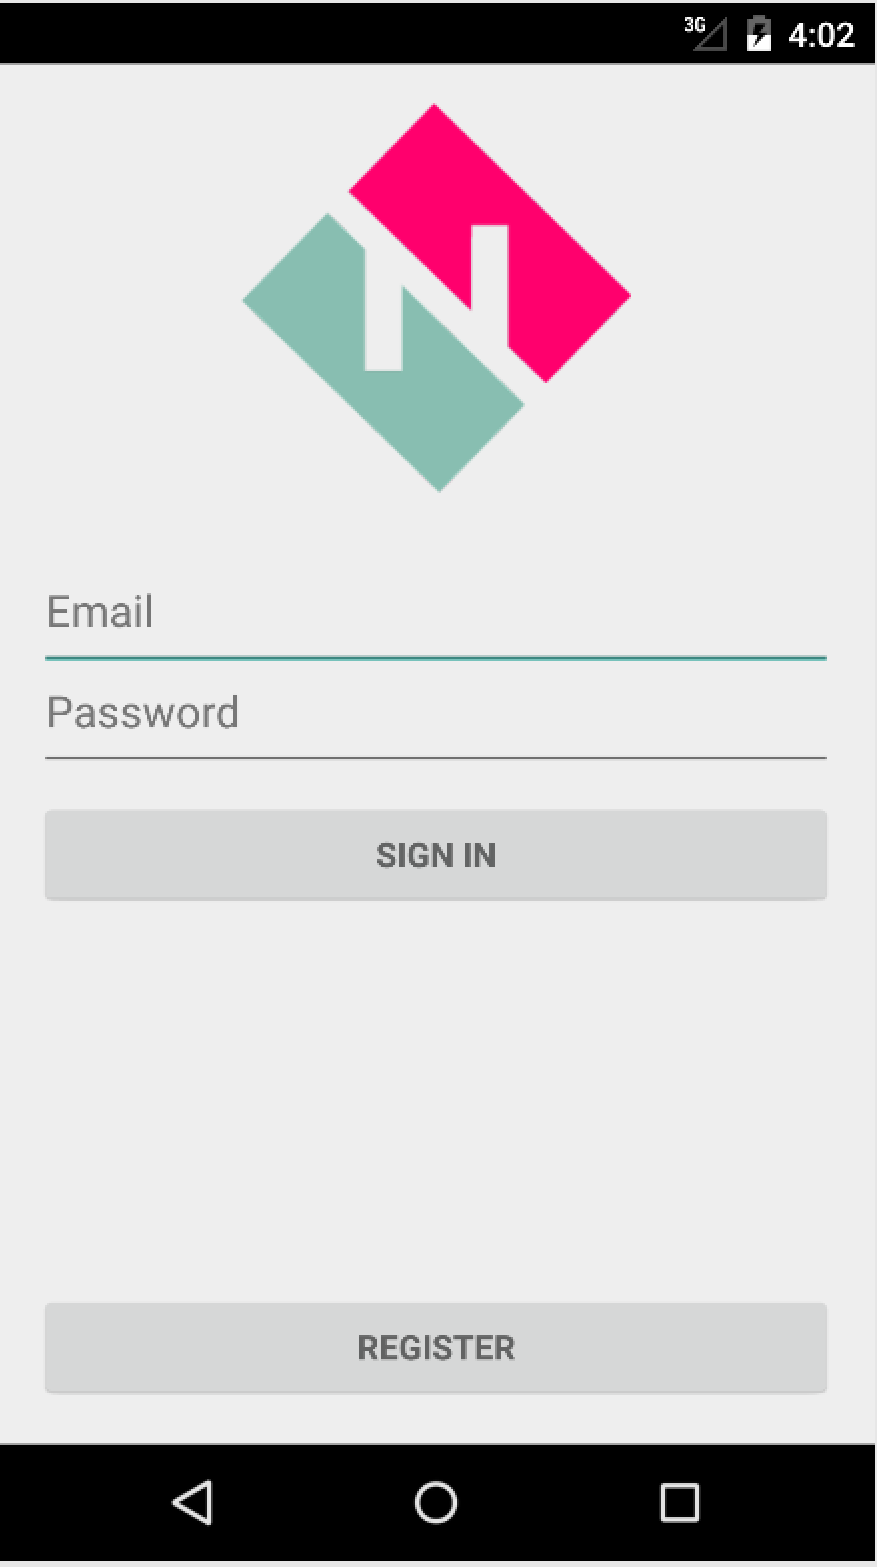
\includegraphics[width=0.9\linewidth]{./Bilder/logIn.png} 
\caption{LogIn Screen}
\label{fig:login}
\end{subfigure}
\begin{subfigure}{0.5\textwidth}
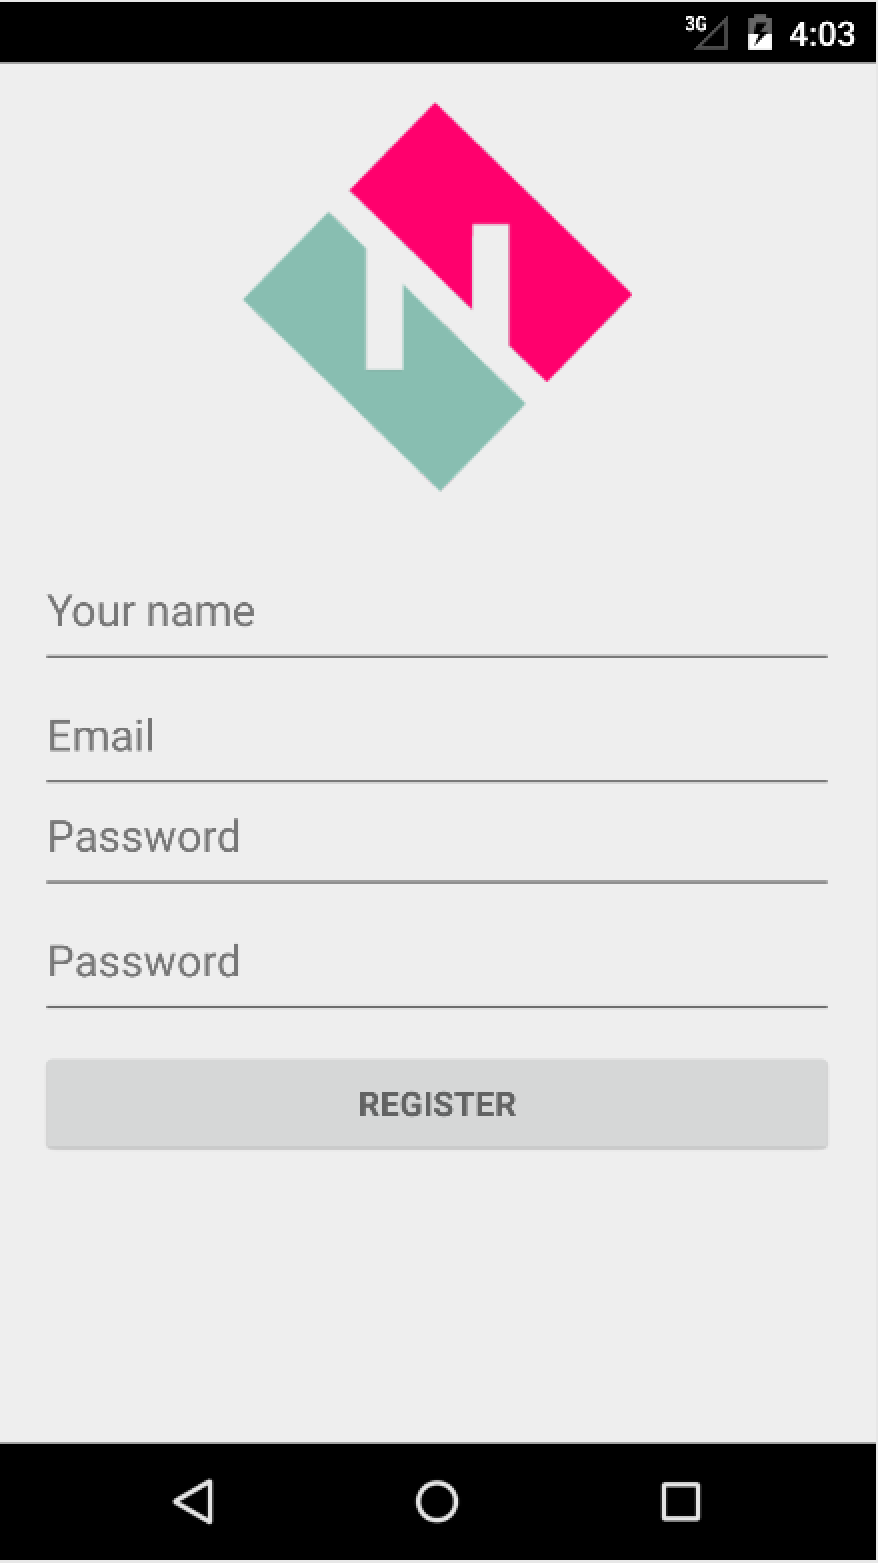
\includegraphics[width=0.9\linewidth]{./Bilder/signUp.png}
\caption{SignUp Screen}
\label{fig:signin}
\end{subfigure}
\caption{}
\label{fig:image2}
\end{figure}

Startet man die App findet man sich zuerst auf einem LogIn/SignUp - Screen wieder. 
Hier kann durch die Eingabe einer g"ultigen Email-adresse und eines Passworts ein Account erstellt, oder sich in einen bestehenden Account eingeloggt werden. 
Die Umsetzung ist schlicht und funktional gehalten. 
Dies kann so "ubernommen werden. 
 
Was erst im Vergleich mit den folgenden Seiten auff"allt, ist dass das Design dieser Seite nicht in das Schema der restlichen App passt. 
Aus Gr"unden der Konsistenz sollte das angepasst werden.

\subsubsection{Start}
\begin{figure}[H]
\begin{center}
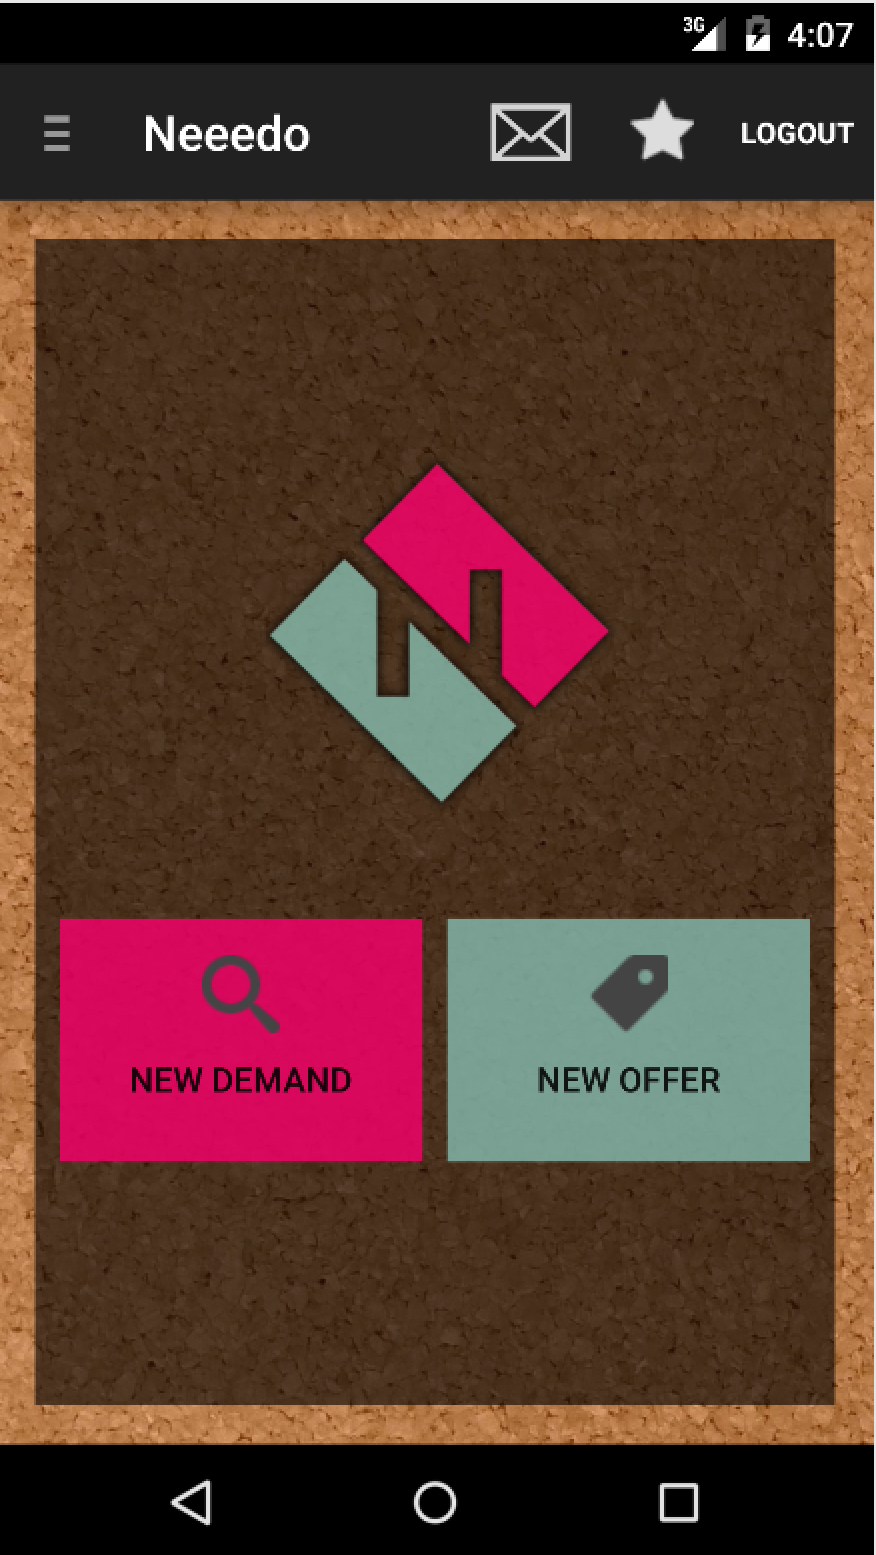
\includegraphics[width=0.45\textwidth]{./Bilder/start.png}
\caption{LandingScreen}
\label{fig:start}
\end{center}
\end{figure}

Loggt man sich in die App ein landet man zuerst auf der hier abgebildeten LandingPage. 
Diese ist schlicht gehalten.
Auf dem halbtransparenten Hintergrund finden sich zwei Button, \enquote{New Demand} und \enquote{New Offer}, die einen wohl zu den Formularen f"uhren mit denen man diese erstellen kann.
Man sieht am oberen Rand des Screens eine Men"uleiste, die einen "BurgerButton" als Men"u, den Schriftzug "Neeedo", ein Briefsymbol als Hinweis auf Nachrichten und einen Logout-Button beinhaltet. 
Dies ist eine (Android-) typische Positionierung f"ur diese  Elemente. 

Der Men"u Button ist dabei der am wenigsten markante Punkt dieses Screens, obwohl man wohl davon ausgehen kann, dass er der Wichtigste ist. 
Der Zugang zum Men"u m"usste markanter sein.

\subsubsection{Men"u}
\begin{figure}[H]
\begin{center}
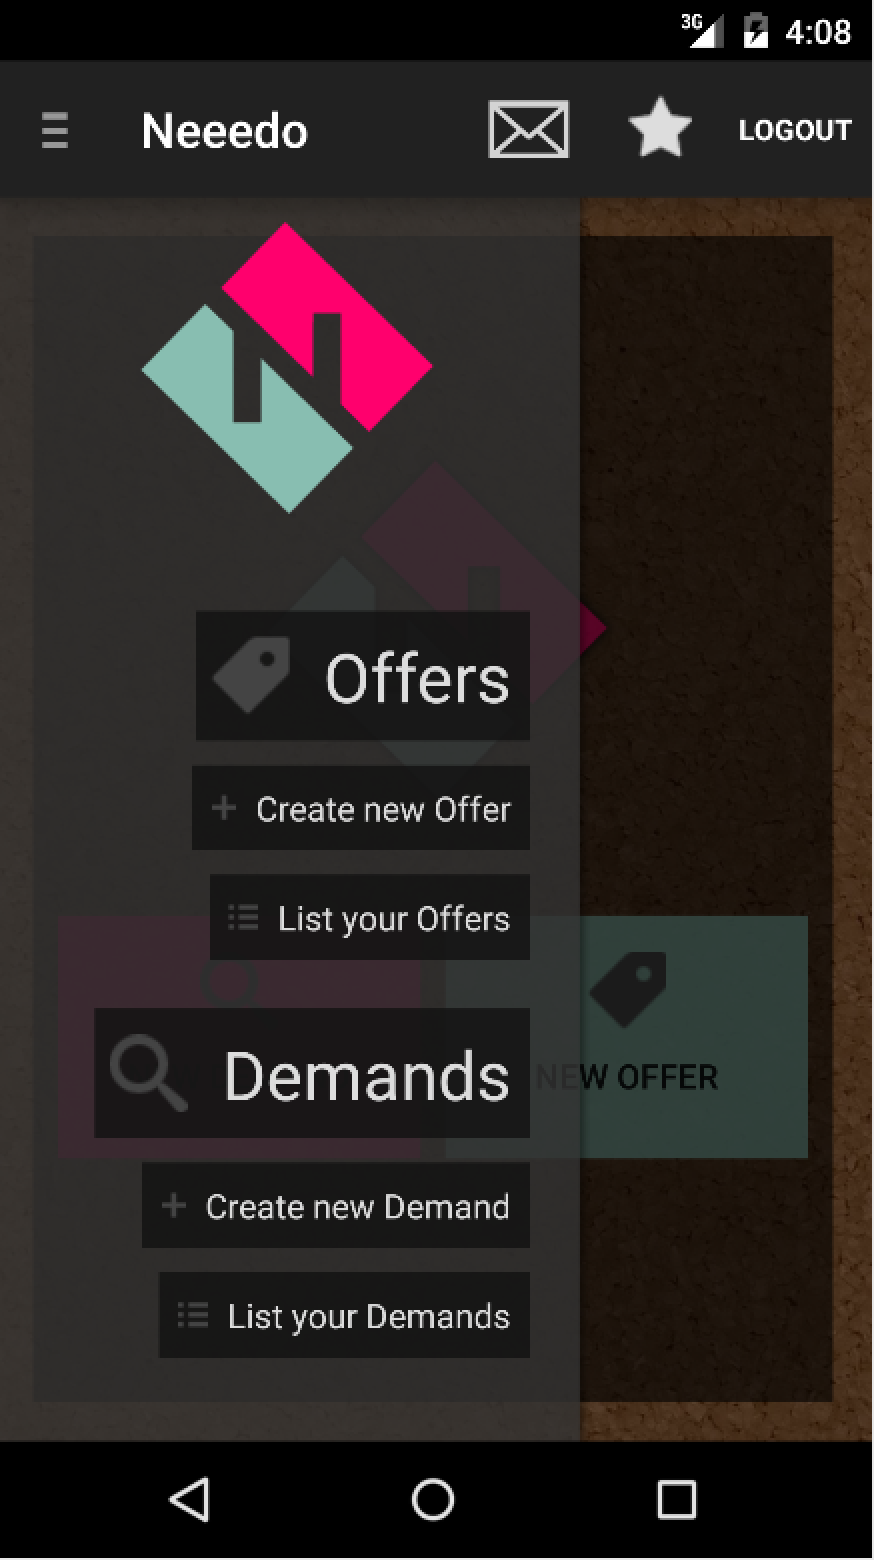
\includegraphics[width=0.45\textwidth]{./Bilder/menu.png}
\caption{Men"u offen}
\label{fig:menu}
\end{center}
\end{figure}

Benutzt man den \enquote{Men"u-Button} "offnet sich das hier abgebildete Men"u.
Dieses bietet, vier Funktionen an: \enquote{Neues Gesuch erstellen}, \enquote{Neues Angebot erstellen}, \enquote{Eigene Angebote auflisten}, \enquote{Eigene Gesuche auflisten}.

Die Umrandung um die Worte, hier, \enquote{Offers} und \enquote{Demands} l"asst vermuten, dass es sich hierbei ebenfalls um Buttons handelt. 
Dies ist jedoch nicht der Fall. 
Es handelt sich hierbei lediglich um Trenner, die das Men"u in drei Sektionen unterteilen.

Betrachtet man sich das Men"u als Ganzes f"allt auf, dass es viel zu viel Platz einnimmt und unn"otig zu sein scheint. 
Um ein solches Men"u zu rechtfertigen m"ssten mehr Funktionen angeboten werden. 

\subsubsection{Agebote und Gesuche erstellen }
\begin{figure}[H]
\begin{subfigure}{0.5\textwidth}
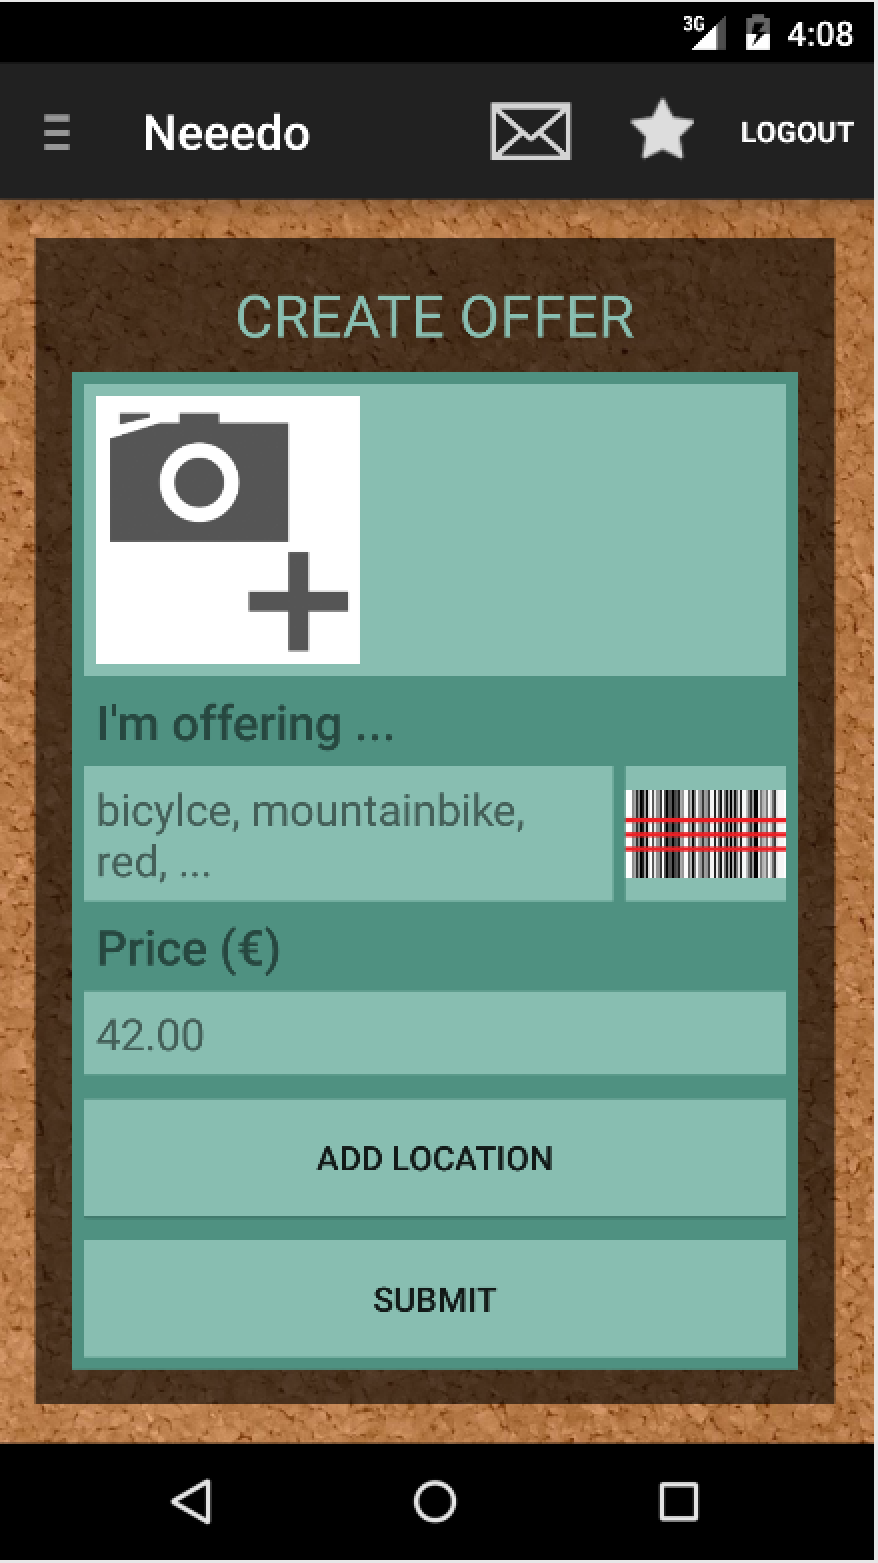
\includegraphics[width=0.9\linewidth]{./Bilder/createOffer.png} 
\caption{Angebot erstellen}
\label{fig:offer}
\end{subfigure}
\begin{subfigure}{0.5\textwidth}
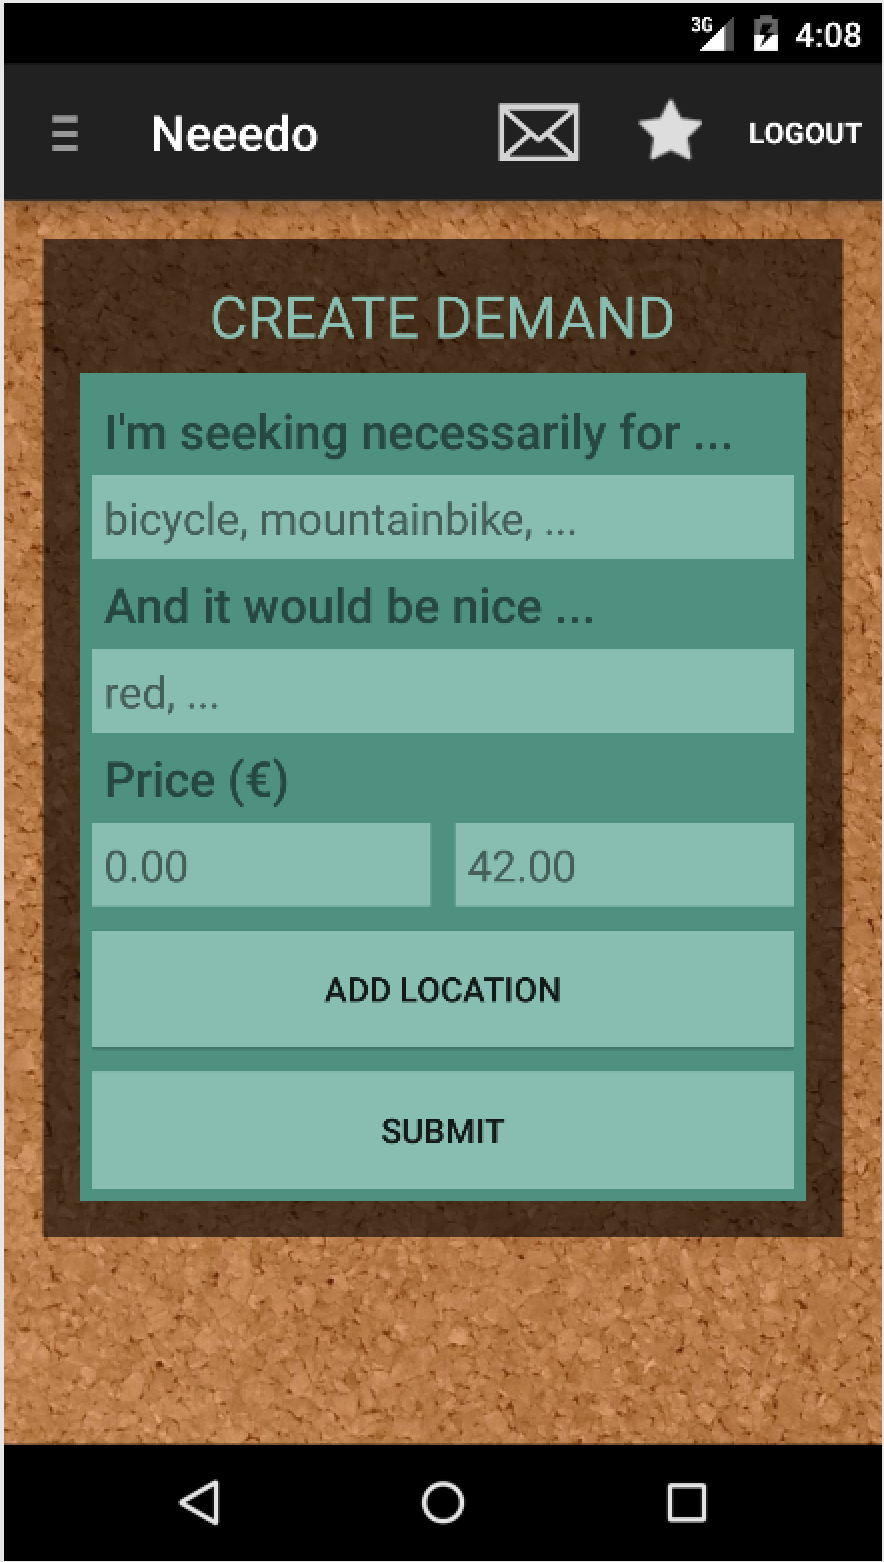
\includegraphics[width=0.9\linewidth]{./Bilder/createDemand.png}
\caption{Gesuch erstellen}
\label{fig:demand}
\end{subfigure}
\caption{}
\label{fig:image4}
\end{figure}

W"ahlt man, entweder im Men"u oder auf dem StartScreen, eine der \enquote{erstellen}-Funktionen aus, landet man auf einer dieser Seiten entsprechend der jeweiligen Auswahl.
Hier wird jeweils ein Formular angezeigt, in dem man eintragen kann was man sucht oder was man anbieten m"ochte. 

Erstellt man ein Angebot/Offer ist es m"oglich Fotos zu hinzuzuf"ugen.
Dies geschieht entweder die Auswahl des Camera-Bildes. 
Dieses ist auf den ersten Blick nicht als Button erkennbar. Dies sollte klarer erkennbar sein. 
Ebenfalls erh"allt man die M"oglichkeit informationen "uber sein Produkt durch das Scannen eines Barcodes zu erhalten. 
Diese Funktionen sind sinnvoll und k"onnten in "ahnlicher Weise "ubernommen werden.

Erstellt man ein Gesuch/Demand, bieter die App keine Zusatzfunktionen an. 
Hier muss das Formular von Hand ausgef"ullt werden.

Beide Formulare besitzen die M"oglichkeit eine Adresse hinzuzuf"ugen, dies geschieht auf einer zus"atzlichen Seite auf der dies durch Auswahl einer Positon auf einer Karte oder ein Suchfeld geschieht.

Befindet man sich auf der Formular-Seite kann man nicht klar erkennen ob man eine Position eingeben muss oder ob es einen Standardwert gibt. 
Dies sollte erkennbar gemacht werden.
 
\subsubsection{Matching}
\begin{figure}[H]
 
\begin{subfigure}{0.5\textwidth}
\includegraphics[width=0.9\linewidth]{./Bilder/matching1.png} 
\caption{Angebot erstellen}
\label{fig:match1}
\end{subfigure}
\begin{subfigure}{0.5\textwidth}
\includegraphics[width=0.9\linewidth]{./Bilder/matching2.png}
\caption{Gesuch erstellen}
\label{fig:match2}
\end{subfigure}
\caption{}
\label{fig:image5}
\end{figure}

Sendet man das auf der \enquote{Gesuch erstellen}-Seite ausgef"ullte Formular ab wird man auf die hier gezeigte \enquote{Matching-View} weitergeleitet. 
Hier werden einem passende Angebote in einer, u.a. aus der App "Tinder" bekannten Stapel-Darstellung pr"sentiert. 
Diese k"onnen entweder durch die Buttons oder durch eine Swipe-Geste nach rechts oder Links verworfen oder als Favorit gespeichert werden. 

Um die gespeicherten Favoriten aufzurufen muss man das Stern-Symbol in der Men"uleiste oben nutzen, im Screen selbst ist keine Weiterleitung m"oglich. 

\subsubsection{\enquote{Eigene} anzeigen}

\begin{figure}[H]
\begin{center}
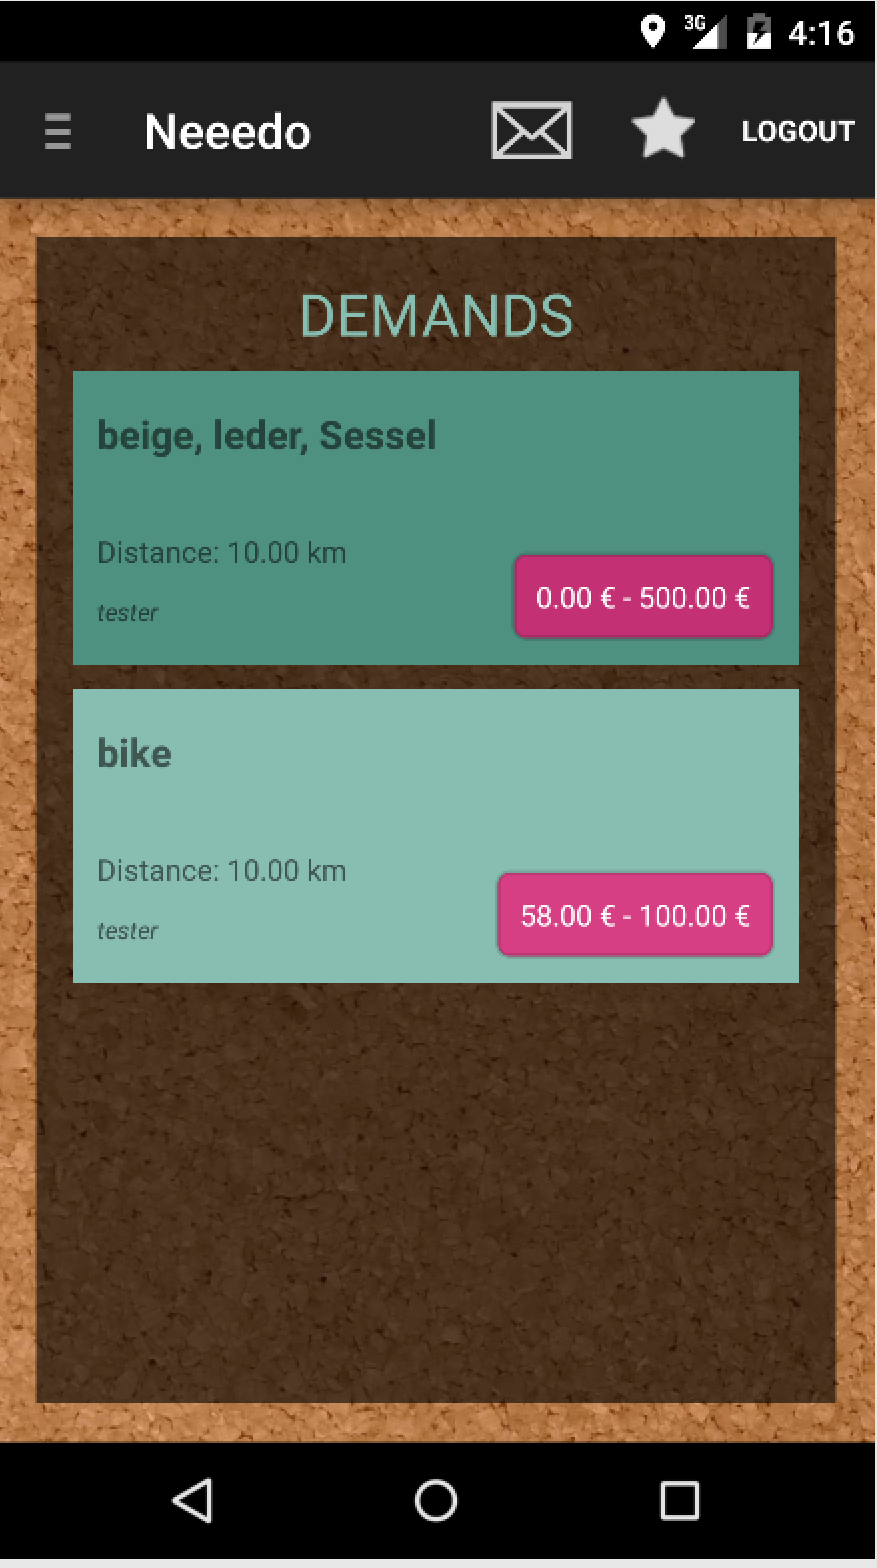
\includegraphics[width=0.45\textwidth]{./Bilder/liste.png}
\caption{Eigene Demands anzeigen}
\label{fig:anzeigen}
\end{center}
\end{figure}

Im Men"u finden sich auch die Funktionen \enquote{eigene Angebote/Gesuche anzeigen}. 
Benutzt man einen dieser Buttons, wird eine Tabelle wie die hier abgebildete pr"asentiert.
Klickt man hier auf eines der aufgef"uhrten Elemente, wird man auf ein Formular "ahnlich dem des \enquote{Erstellens} geleitet, auf dem "Anderungen durchgef"uhrt werden k"onnen. 

\subsection{Fazit}

Dies sind die wichtigsten Funktionen dieser App, weitere wie zum Beispiel der Versand von Nachrichten werden nicht n"aher betrachtet, da hier nur ein Standard Chat zum Einsatz kommt. 

\subsubsection{Positiv}\begin{description}
\item[+] Das Design ist einheitlich 
\item[+] Viele Funktionen k"onnen "ubernommen werden
\end{description}

\subsubsection{Negativ}\begin{description}
\item[-] Nicht alle Buttons k"onnen als solche erkannt werden
\item[-] Elemente k"onnen irrt"umlich f"ur Buttons gehalten werden.
\item[-] Seitenmen"u zu gro"s und unpraktisch 
\item[-] Login nicht im selben Design
\end{description}

